\section*{Terrain Generation}
When designing the way the terrain is randomly generated so that we can have a new, unique map every time we play.
The second thing we wanted was to make sure that the player could edit the terrain in any way they wanted.
These two requirements made us decide on the algorithm described in this section.

The algorithm consists of the following steps:
\begin{itemize}
    \item Generate a scalar field for the whole world.
    \item Divide the world into chunks.
    \item Generate the terrain.
\end{itemize}

Each of these steps will be described in more detail alter in this section.

\subsection*{Scalar Field} \label{subsec:scalar_field}
The first step in the terrain generation is to generate a scalar field which is a function that takes a point in 3D space and returns a value.
What is important is that this function always returns the same value for the same point.
Another important feature is that the function should return close values for close points.
Our function returns values for points which have integer coordinates.

Having these properties in mind we decided to use the Perlin noise function.
Perlin noise first introduced by Ken Perlin in 1983 \cite{perlin_noise} is often used in computer graphics and in particular in procedural terrain generation.
It is a pseudo-random function that returns random values any point in 3D space.
However unlike other random functions it returns similar values for similar points.
This makes it ideal for this game.

The Perlin noise function is used to generate a value for each point in the scalar field.
This value is then modified based on 5 parameters: octaves, initial frequency, frequency multiplier, initial amplitude and amplitude multiplier.
These parameters are generate based on the seed of the world from 5 different sets of options which gives the game 5 terrains.
However we need more than just the value for each point.
Each point is also assigned a type based on the position that is later used to determine the type of the block which in turn determines its color.
The color
\subsection*{Chunks}
As mentioned before one of the most important thinks for the terrain was a way to edit it.
Editing the whole terrain at once would be very slow and not very efficient.
Thus the terrain is split into chunks - cubes with side length 16.
Each chunk is a separate object and can be edited independently.
This solution is much more efficient but is also has some problems.

One problem is that the terrain is not continuous.
Every time we edit a chunk we need to make sure that the edges of the chunk are the same as the edges of the neighboring chunks.
This is done by making sure that when a function that updates one chunk is called it is also called with the exact same parameters for other affected chunks.
Without this the terrain would have holes in it between chunks which is shown in a screenshot from an early version of the game in \autoref*{fig:gaps_between_chunks}.

Another problem is that the algorithm we used for generating the terrain, described in \autoref*{subsec:marching_cubes}, calculates normal vectors based on the values of the scalar field around the point at which the normal is calculated.
This means that that the normal vectors at the edges of the chunks have to be calculated differently.
This is a common problem with the algorithm and it is visualized in \autoref*{fig:problem_with_normals_at_chunk_edge}.
The most common solution and the one we used is extending the scalar field by one layer of points around the chunk.
This means that the chunk contains the information about the scalar field outside of the chunk itself.
That way the normal vectors can be calculated the same way for all points in the chunk.

\begin{figure}[H]
    \centering
    \begin{minipage}{0.45\textwidth}
        \centering
        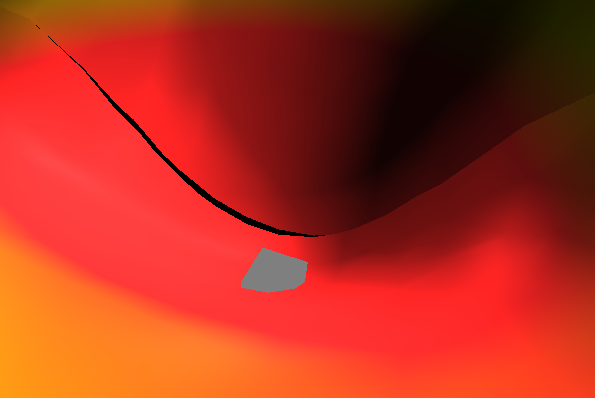
\includegraphics[width=0.8\textwidth]{chapters/terrain_generation/resources/chunk_edges_gaps.png}
        \caption{Gaps between chunks.}
        \label{fig:gaps_between_chunks}
    \end{minipage}\hfill
    \begin{minipage}{0.45\textwidth}
        \centering
        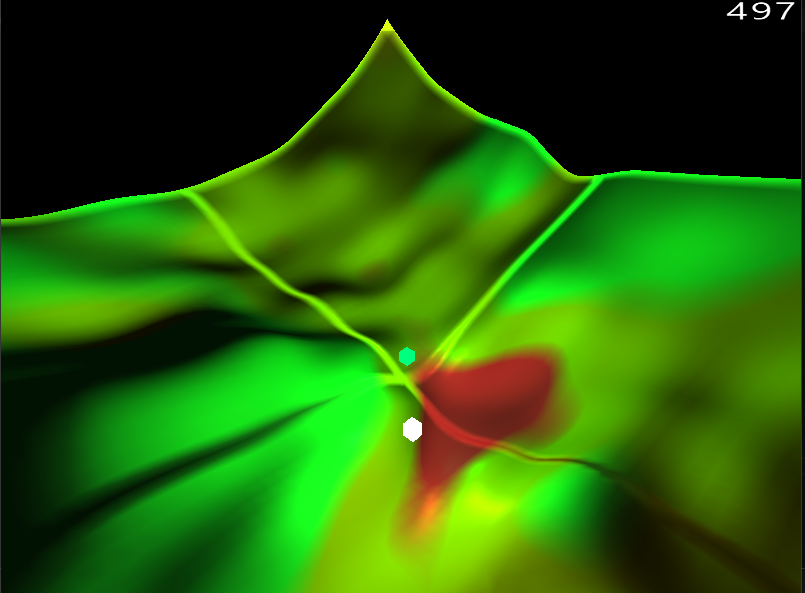
\includegraphics[width=0.8\textwidth]{chapters/terrain_generation/resources/chunk_edges_normals_problem.png}
        \caption{Problem with normals at chunk edges.}
        \label{fig:problem_with_normals_at_chunk_edge}
    \end{minipage}
\end{figure}
\subsection*{Marching Cubes} \label{subsec:marching_cubes}
Marching cubes is an algorithm for generating a 3D mesh from a scalar field.
It was first described by William E. Lorensen and Harvey E. Cline in 1987 \cite{marching_cubes}.
The main idea behind the algorithm is to divide the scalar field into cubes and then generate a mesh for each one of them.

Some isolevel is chosen and then each point that has a value greater than the isolevel is considered to be "above" the surface and each point with a value lower than the isolevel is considered to be "below" the surface.
We know that a surface has to separate the points that are above it from the points that are below it.
Every cube has 8 vertices and each vertex is either above or below the surface which gives us a total of 256 combinations (some combinations being rotations of others).
For each of these combinations we use a precomputed table to generate a mesh.
The table tells us which edges of the cube are intersected by the surface and how to connect them.
To make the mesh look smoother we interpolate the position of the vertices on the edges based on the values of the scalar field at the vertices.
This is done by using the linear interpolation. % Maybe add formula here?
This gives us a mesh.

However to make the mesh look even smoother we also need to calculate the normal vectors for each vertex.
The normal vectors for each vertex of the scalar field are calculated using \autoref*{eq:normal_vector}
\begin{equation}
    \label{eq:normal_vector}
    n(x, y, z) = \begin{bmatrix}
        s(x + 1, y, z) - s(x - 1, y, z) \\
        s(x, y + 1, z) - s(x, y - 1, z) \\
        s(x, y, z + 1) - s(x, y, z - 1)
      \end{bmatrix}
\end{equation}
where $s$ is the scalar field and $n$ is the normal vector.
These vectors are used to calculate the mesh normals using the same interpolation used for the mesh.

Last part of creating the mesh is assigning the colors to each vertex.
Each vertex of the scalar field is assigned a type which is described in \autoref*{subsec:scalar_field}.
Each type has a color assigned to it.
The color of each vertex of the mesh is calculated by interpolating the colors of the vertices of the scalar field.


